\section{\vita: Challenges and design goal}
\label{sec:example}
\todo{Borrow the Teddy usecase as example. Drop data mangement challenges like C3 and C5. Drop D3 and D5.}

\stitle{Motivating Example.} 
Ada, a data scientist in the e-commerce department of a retail business, has been tasked to analyze customer reviews of products purchased from their website. Ada would like to capture the underlying topics by performing topic modeling and clustering to characterize the review corpus better. Figure~\ref{fig:workflow} captures the use-case which involves---(a) preprocessing the data (\emph{clean}), creating feature vectors from the text reviews (\emph{featurize}), creating topic vectors from the corpus (\emph{topic modeling}), clustering reviews into topics (\emph{cluster assignment}), and finally, visualizing the clusters by projecting the topics vectors to lower dimensions (2D) using feature transformation techniques such as PCA (\emph{visualize}). In practice, the workflow may be non-linear, and each step may require multiple passes and different tools. In the process, visualizations are useful not only for exploratory analysis or final presentation but also for every other step---\vita workflows resemble the \emph{read-eval-print loop} (REPL) approach where users perform incremental operations on data and examine intermediate results. We now characterize the challenges of the existing \vita  workflows in the context of this use-case as follows:


\todo{If applicable, consider revising the names of challenges to sound more like challenges, less like design goals or criteria.} 

\todo{Consider combining  C1 and C3} 

\todo{Maybe, "C1. Overhead due to data and workflow heterogeneity"?} 

\emtitle{C1. Workflow discontinuity.}As mentioned in Section~\ref{sec:intro}, data scientists lack tools 
that support different \vita operations and workflows within an integrated environment.
For example, to define the data cleaning rules, Ada first visually inspects the data using tools like spreadsheets. Next, they execute those rules in a computational notebook, \eg Jupyter. Upon inspecting the data in the spreadsheet, Ada may revise the rules in the notebook. To visualize top-ranked words after the featurization step (\eg a bar chart of words ranked by their TF-IDF scores), they need to either use dedicated visualization tools or write scripts in the notebook. Therefore, even completing simple tasks may require accessing different tools, which can be cumbersome user experience due to, for example, the logistical and cognitive overhead of context switching.
 
\todo{Maybe, "C2. Tension between interactivity and extensibility"?}


\emtitle{C2. Limited coordination.}  \vita necessitates coordination among different views (\eg between visualization and raw data).  The high dimensional text data can be difficult to interpret and users often map different facets of the data to visualizations for better interpretability. 
However, without coordination between perceptual components and the data space, understanding the relations between the facets of the same entities on demand can be challenging. 
For example, say Ada wants to inspect which reviews contain a top-word shown in a  bar chart (generated after featurization). However, visualizations in notebooks or visualization tools are decoupled from the data. As a result, Ada has to either open and then filter the data in a spreadsheet, or programmatically filter the data from the notebook to inspect the relevant reviews. Therefore, the lack of coordination impacts both workflow continuity and the user's ability to explore data effectively.
 


\begin{figure}[tbp] 
%  \vspace{-10pt}
  \centering
  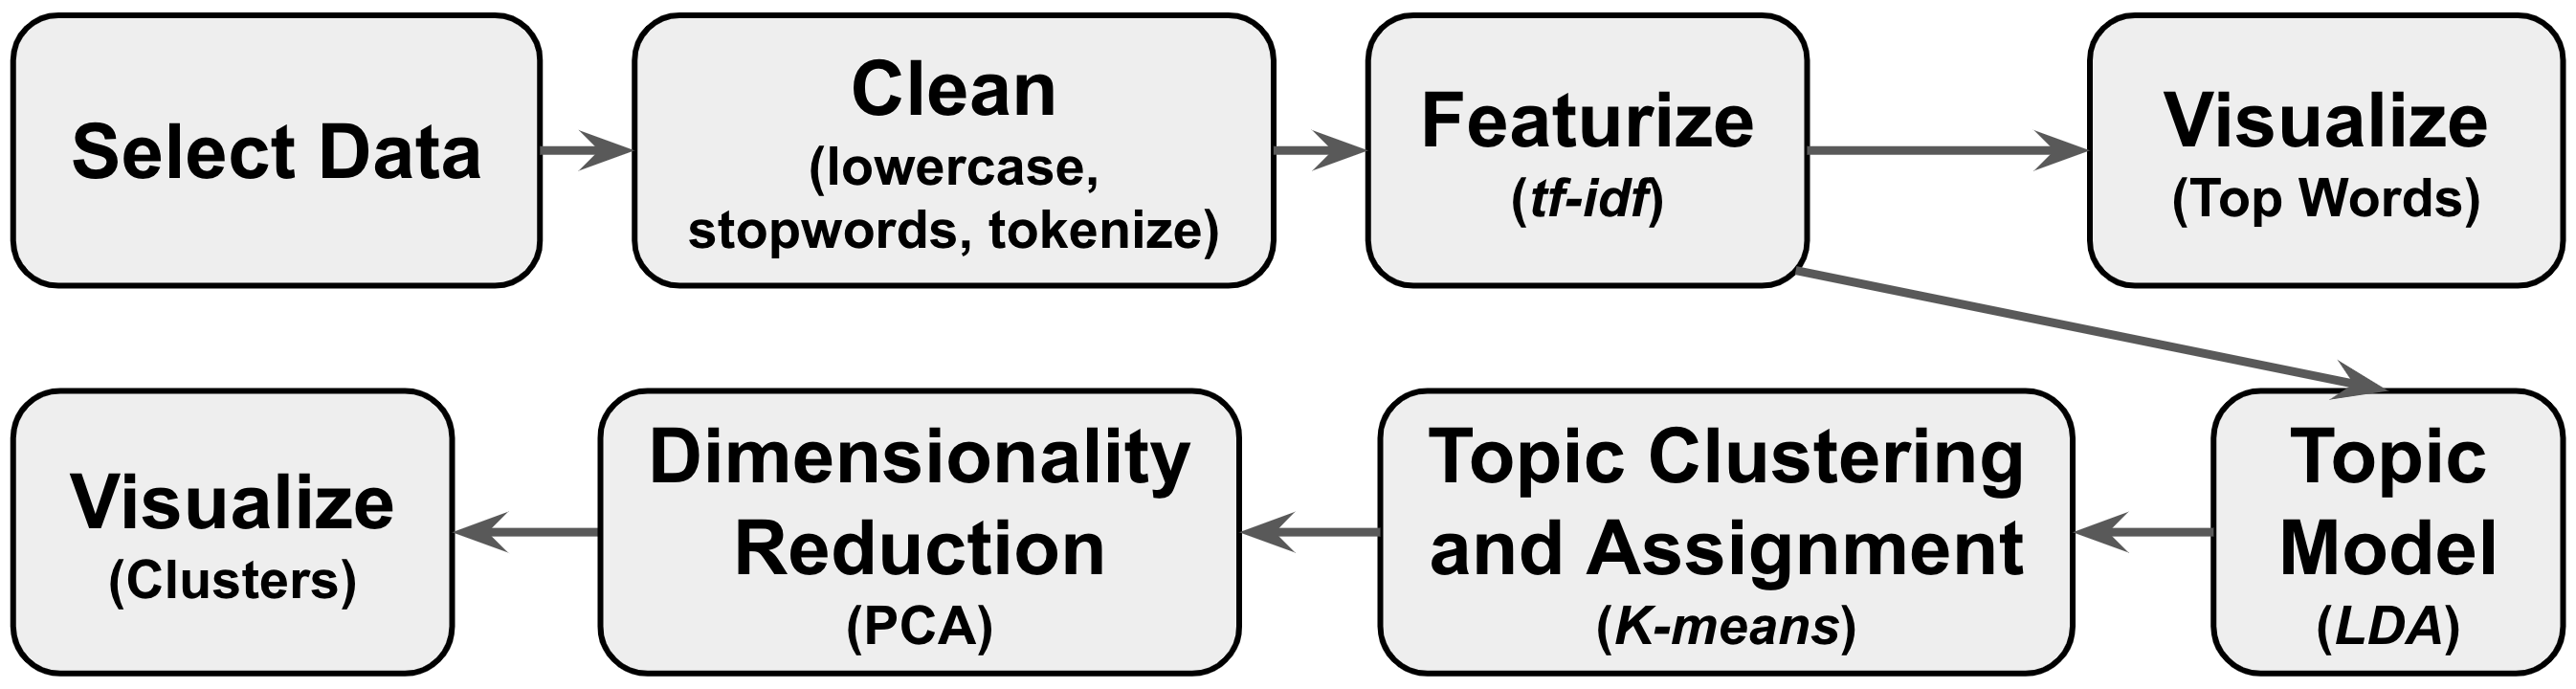
\includegraphics[width=\linewidth]{figures/workflow.png}
  \caption{\small An example \vita use-case: topic exploration.\label{fig:workflow}} 
  \vspace{-20pt}
\end{figure}

\emtitle{C3. Data types and workflow diversity.} \vita workflows deal with heterogeneous data (\eg text, visualizations) and workflows (\eg in use-cases like text summarization, sentiment analysis). While there are a number of \vita tools for specific workflows~\cite{liu2018bridging}, more often than not these tools use a stack of independent solutions for data storage and
processing glued together by scripting languages like Python and R.
These bespoke solutions typically don’t support direct data manipulation and interactive visual coordination. As a result, users are often forced to develop new and heavily customized systems on top of these solutions.

\emtitle{C4. On demand workflow authoring.} 
\vita workflows contain a variety of operations, \eg cleaning, featurization, interactive visualization, classification. Similar to relational~\cite{codd} or data visualization algebra~\cite{satyanarayan2016vega}, \vita operations with similar objectives can be grouped into high-level categories. Moreover, operations in different categories can be combined to compose new operation pipelines. For example, cleaning and featurization can be combined into a preprocessing pipeline. As existing systems lack any formalization of the operations and their application, the onus is on the user to design the optimal analytics workflow for different use-cases.

\emtitle{C5. \vita Session management.} As demonstrated in the usage example, \vita workflows warrant the trial-and-error style  iterative approach---users often need to reproduce previous steps of the workflow, make updates, and rerun the subsequent steps. 
Therefore, ensuring reproducibility of  \vita sessions requires management of dataset versions produced by various operations, the operation logs, and different states of and interactions on the visual representations of the data. 
Prior work from the data management community focused on versioning structured datasets~\cite{huang2017orpheusdb}, versioning code for debugging workflows~\cite{brachmannbyour,miao2016provdb} and managing deep learning models~\cite{miao2016modelhub}.
However, these systems lack support for versioning an end-to-end \vita workflow involving heterogeneous data types and user interactions spanning multiple views. 

